\begin{figure}[H]
    \centering
    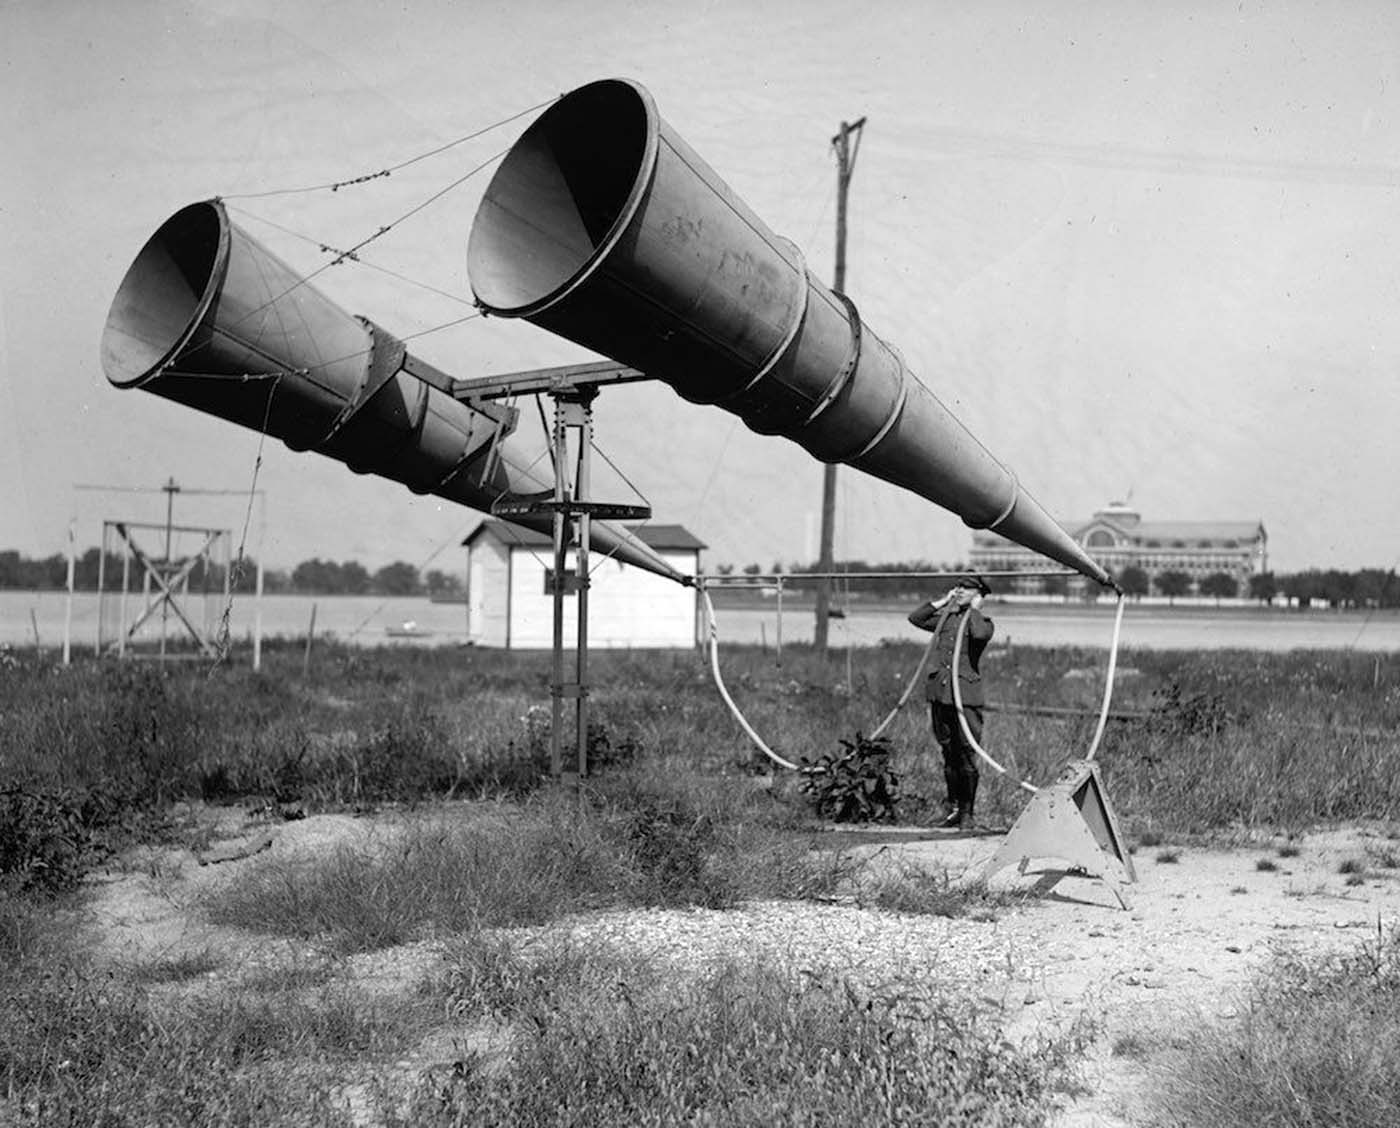
\includegraphics[width=1\textwidth]{Figures/acousticloc.jpg}
    \label{fig:acousticloc}
\end{figure}

\thispagestyle{empty}
{\small
\strut\vfill % push the content to the bottom of the page
\noindent Copyright \copyright{} Aalborg University 2018\par
\vspace{0.2cm}
\noindent This report has been compiled using \LaTeX.
}
\clearpage

\newpage
\pdfbookmark[0]{English title page}{label:titlepage_en}
\aautitlepage{%
  \englishprojectinfo{
    Outdoor Sound Localization using a tetrahedral microphone array %title
  }{%
    Master's Thesis %theme
  }{%
    Fall Semester 2018 %project period
  }{%
    AAT10-1062 % project group
  }{%
    %list of group members
    Ashwin Saraf\\ 
    Maxime Démurger
  }{%
    %list of supervisors
    Søren Krarup Olesen\\
  }{%
    1 % number of printed copies
  }{%
    \today % date of completion
  }%
}{%department and address
  \textbf{Electronics and IT}\\
  Aalborg University\\
  \href{http://www.aau.dk}{http://www.aau.dk}
}{% the abstract
   The impact of sound on individual's health can be dramatic when one is exposed to high sound pressure level (SPL) for a long period of time. While SPL at concerts are measurable using one microphone, it can be difficult to do the same in outdoor environments when multiple sources are present. This work aims at developing a monitoring system to localize the main outdoor noise contributors while retrieving their SPL. Using signal processing and a microphone array to capture the sound, it is possible to compute a sound map of the array surroundings. Sound localization techniques have been implemented successfully in a wide range of product, notably the SRP-PHAT algorithm which combines the beamforming techniques and time difference of arrival (TDOA) information. However this method is designed for sources in a reverberant field while the outdoor environment is sensibly different. This works improves the robustness of SRP-PHAT for outdoor sound localization and present a method to deconvolve the array response from the result. This new algorithm, the MP-SRP-PHAT is presented and experimentally evaluated in various conditions. The algorithm improves SRP-PHAT when multiple sources are present on the map however it cannot handle coherent sources.
  
}
